%%%%%%%%%%%%%%%%%%%%%%%%%%%%%%%%%%%%%%%%%
% University/School Laboratory Report
% LaTeX Template
% Version 3.1 (25/3/14)
%
% This template has been downloaded from:
% http://www.LaTeXTemplates.com
%
% Original author:
% Linux and Unix Users Group at Virginia Tech Wiki 
% (https://vtluug.org/wiki/Example_LaTeX_chem_lab_report)
%
% License:
% CC BY-NC-SA 3.0 (http://creativecommons.org/licenses/by-nc-sa/3.0/)
%
%%%%%%%%%%%%%%%%%%%%%%%%%%%%%%%%%%%%%%%%%

%----------------------------------------------------------------------------------------
%	PACKAGES AND DOCUMENT CONFIGURATIONS
%----------------------------------------------------------------------------------------

\documentclass{article}

\usepackage{graphicx} % Required for the inclusion of images
\usepackage{amsmath} % Required for some math elements 
\usepackage{cite}
\usepackage{subcaption} %Required to group figures
\usepackage{float}

\setlength\parindent{0pt} % Removes all indentation from paragraphs

%\usepackage{times} % Uncomment to use the Times New Roman font

%----------------------------------------------------------------------------------------
%	DOCUMENT INFORMATION
%----------------------------------------------------------------------------------------

\title{Lab 5\\ Baseband PAM\\ EE 445S} % Title

\author{Enoc Balderas\\
        \and
        Daniel Diamont\\} % Author name

\date{\today} % Date for the report

\begin{document}

\maketitle % Insert the title, author and date

\begin{center}
\begin{tabular}{l r}
Date Performed: & March 1, 2019 \\ % Date the experiment was performed
Instructor: & Professor Evans % Instructor/supervisor
\end{tabular}
\end{center}

% If you wish to include an abstract, uncomment the lines below
% \begin{abstract}
% Abstract text
% \end{abstract}

%----------------------------------------------------------------------------------------
%	SECTION 1
%----------------------------------------------------------------------------------------

\section{Introduction}

For this  lab we experimented with the FIR and IIR filter design process.
We started off by using MATLAB's fdatool to experiment with different filter designs, and to gain intuition about the rules of thumb for meeting filter specifications.
Additionally we plotted the filter magnitude and phase to verify that the specifications have been met.
Finally we used the filter coefficients generated from MATLAB to implement IIR and FIR filters in C on our DSP board.

\subsection{Pulse Shaping}

We experimented with both sample based processing and frame based processing.
Within our sample based implementation we tested the difference in speed between a linear buffer and a circular buffer.
We also compared our sample based circular buffer implementation to a frame based processing implementation and compared the tradeoffs between them.

\subsection{SCR}

We experimented with a direct form II implementation and also a cascade of second order biquads.
We compared the implementation complexity of both methods and the number of coefficients required for each.
For instance biquads are reusable logic blocks, but there is lots of programming overhead setting up the biquad implementation.

\subsection{Demodulation}


%----------------------------------------------------------------------------------------
%	SECTION 2
%----------------------------------------------------------------------------------------

\section{Methods}

\subsection{Linear and Circular buffering}

We designed a 30th order FIR filter in MATLAB and recorded its magnitude response for frequencies between 1 - 24 kHz.
After confirming the response in MATLAB we exported the filter coefficients to a C file for implementation on DSP board.
On the DSP board we tested the clock cycles spent with both linear and circular buffers.

\subsection{Frame based processing}

Using the same FIR filter coefficients we experimented with a frame based approach and compared the results to the circular buffer sample based implementation.
We also experimented with the compiler optomizations available in CCS for a convolution method written in C compared to one in assebly.

\subsection{IIR filtering}

We designed a 6th order IIR filter in MATLAB and recorded its magnitude response for frequencies between 1 - 24 kHz.
After confirming the response in MATLAB we exported the filter coefficients to a C file for implementation on DSP board.
We compared the performance of the direct form implementation with a second order biquad cascade.
 
%----------------------------------------------------------------------------------------
%	SECTION 3
%----------------------------------------------------------------------------------------

\section{Results}

\subsection{Pulse Shaping}

\begin{figure}[h]
  \begin{center}
    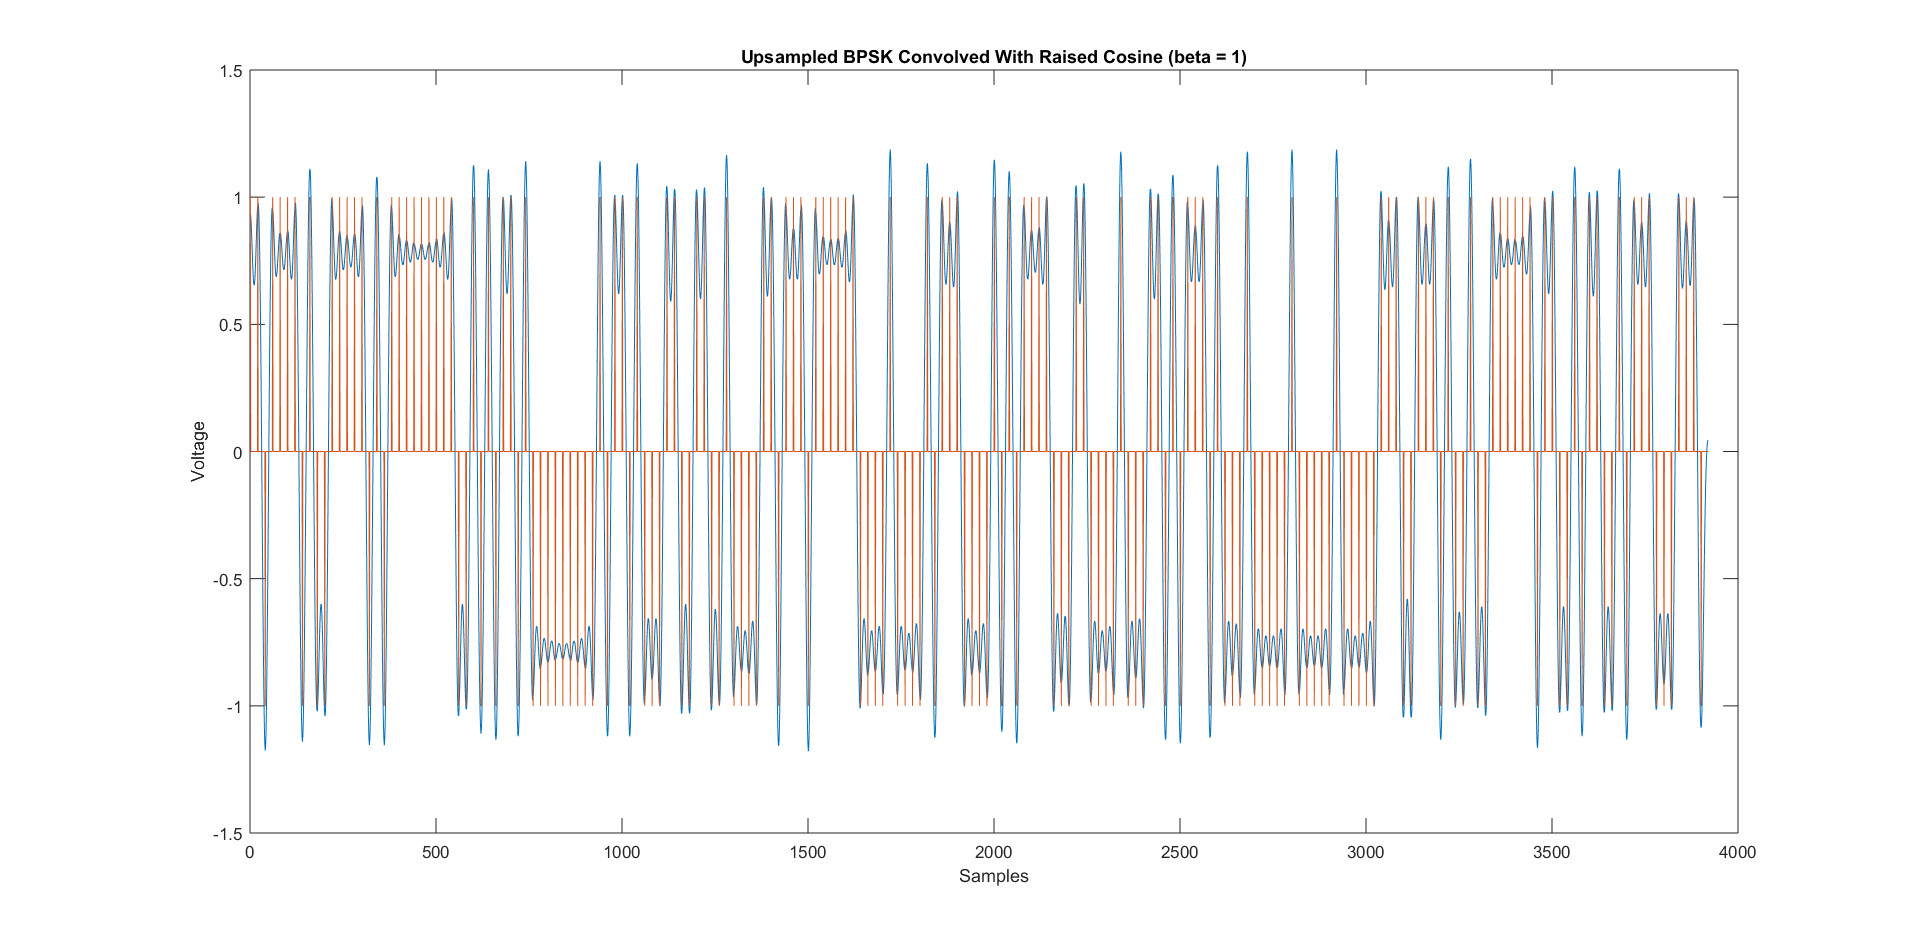
\includegraphics[width=0.65\textwidth]{img/upsampled_bpsk_raised_cosine_beta_1.png}
    \caption{Pulse shape BPSK $\beta = 1$.}
  \end{center}
\end{figure}

\begin{figure}[h]
  \begin{center}
    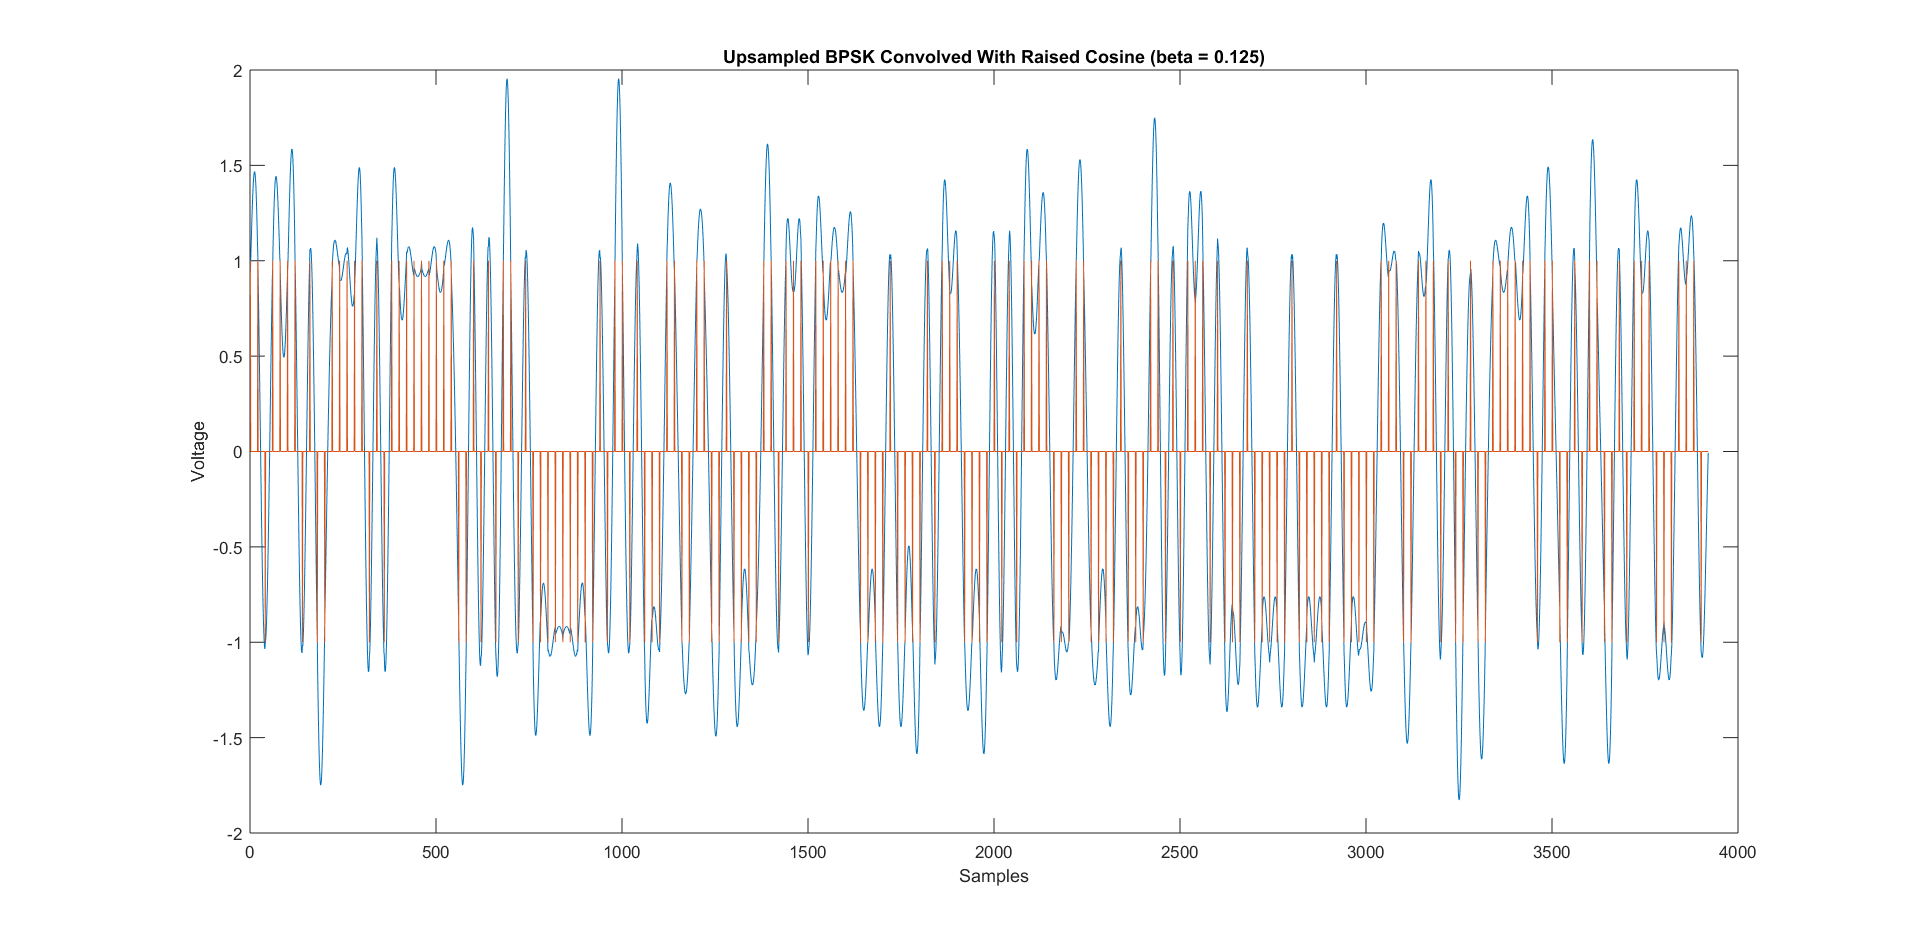
\includegraphics[width=0.65\textwidth]{img/upsampled_bpsk_raised_cosine_beta_125.png}
    \caption{Pulse shape BPSK $\beta = 0.125$.}
  \end{center}
\end{figure}

\begin{figure}[h]
  \begin{center}
    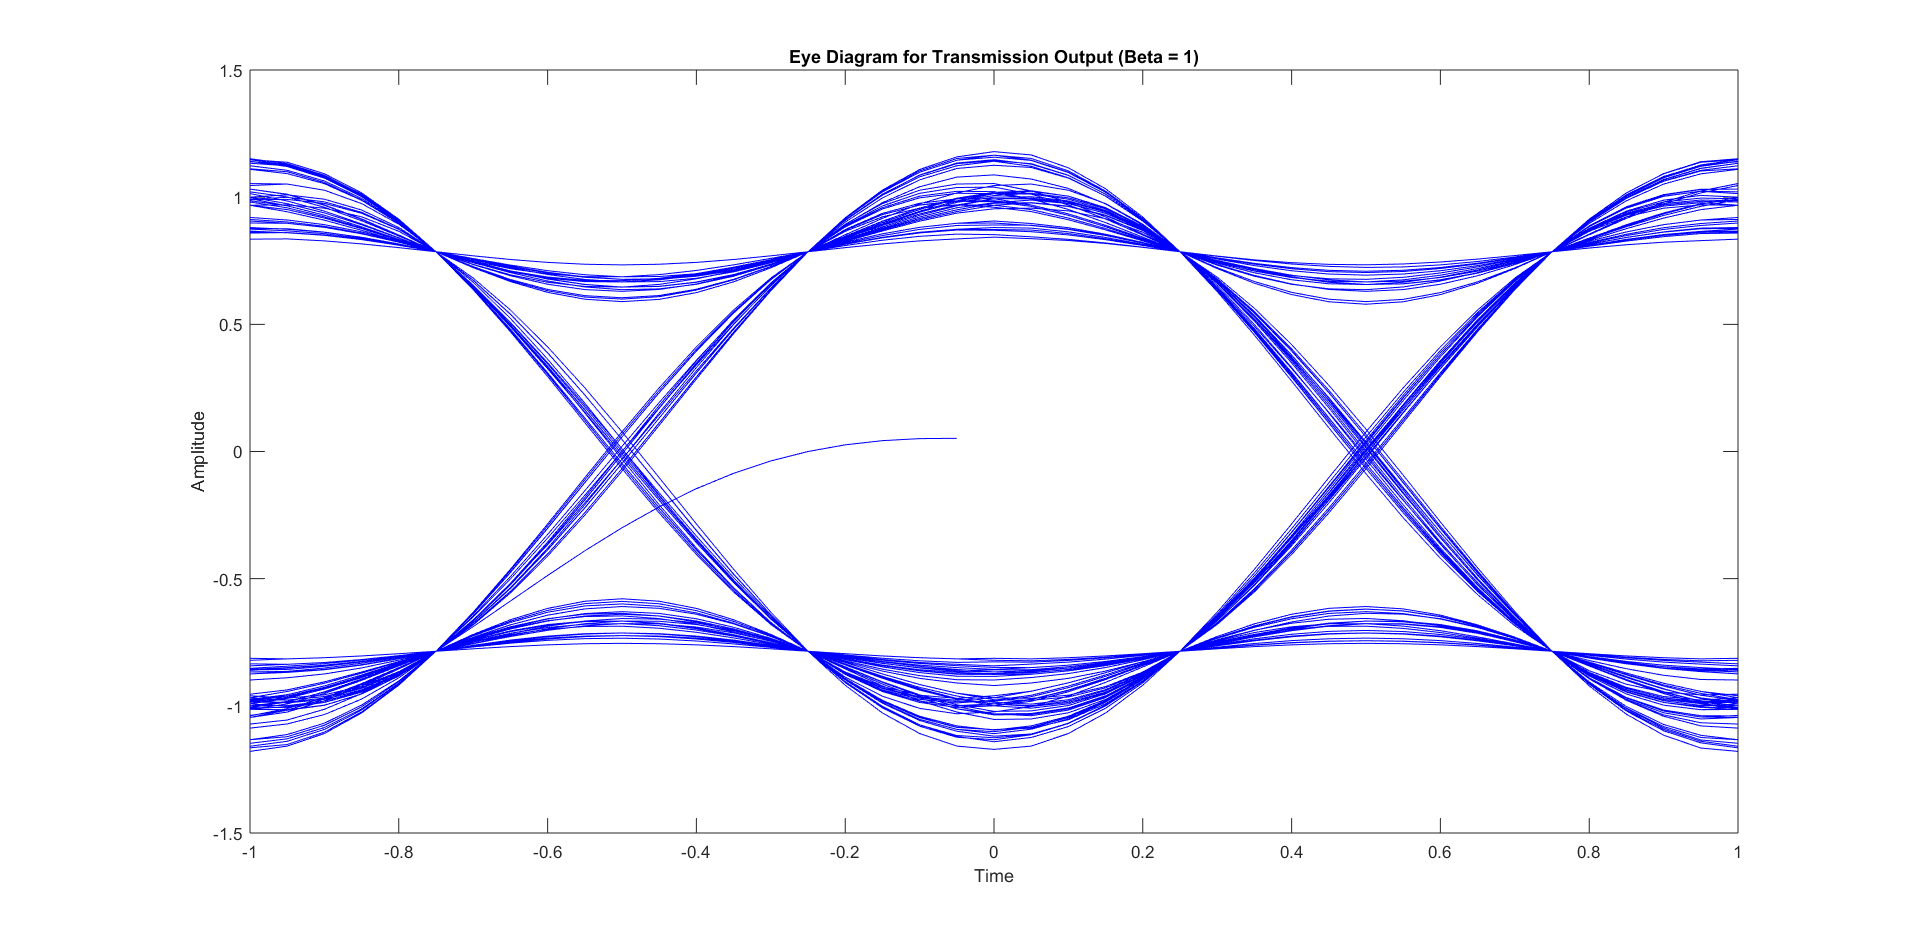
\includegraphics[width=0.65\textwidth]{img/eye_diagram_beta_1.png}
    \caption{Eye diagram $\beta = 1$}
  \end{center}
\end{figure}

\begin{figure}[h]
  \begin{center}
    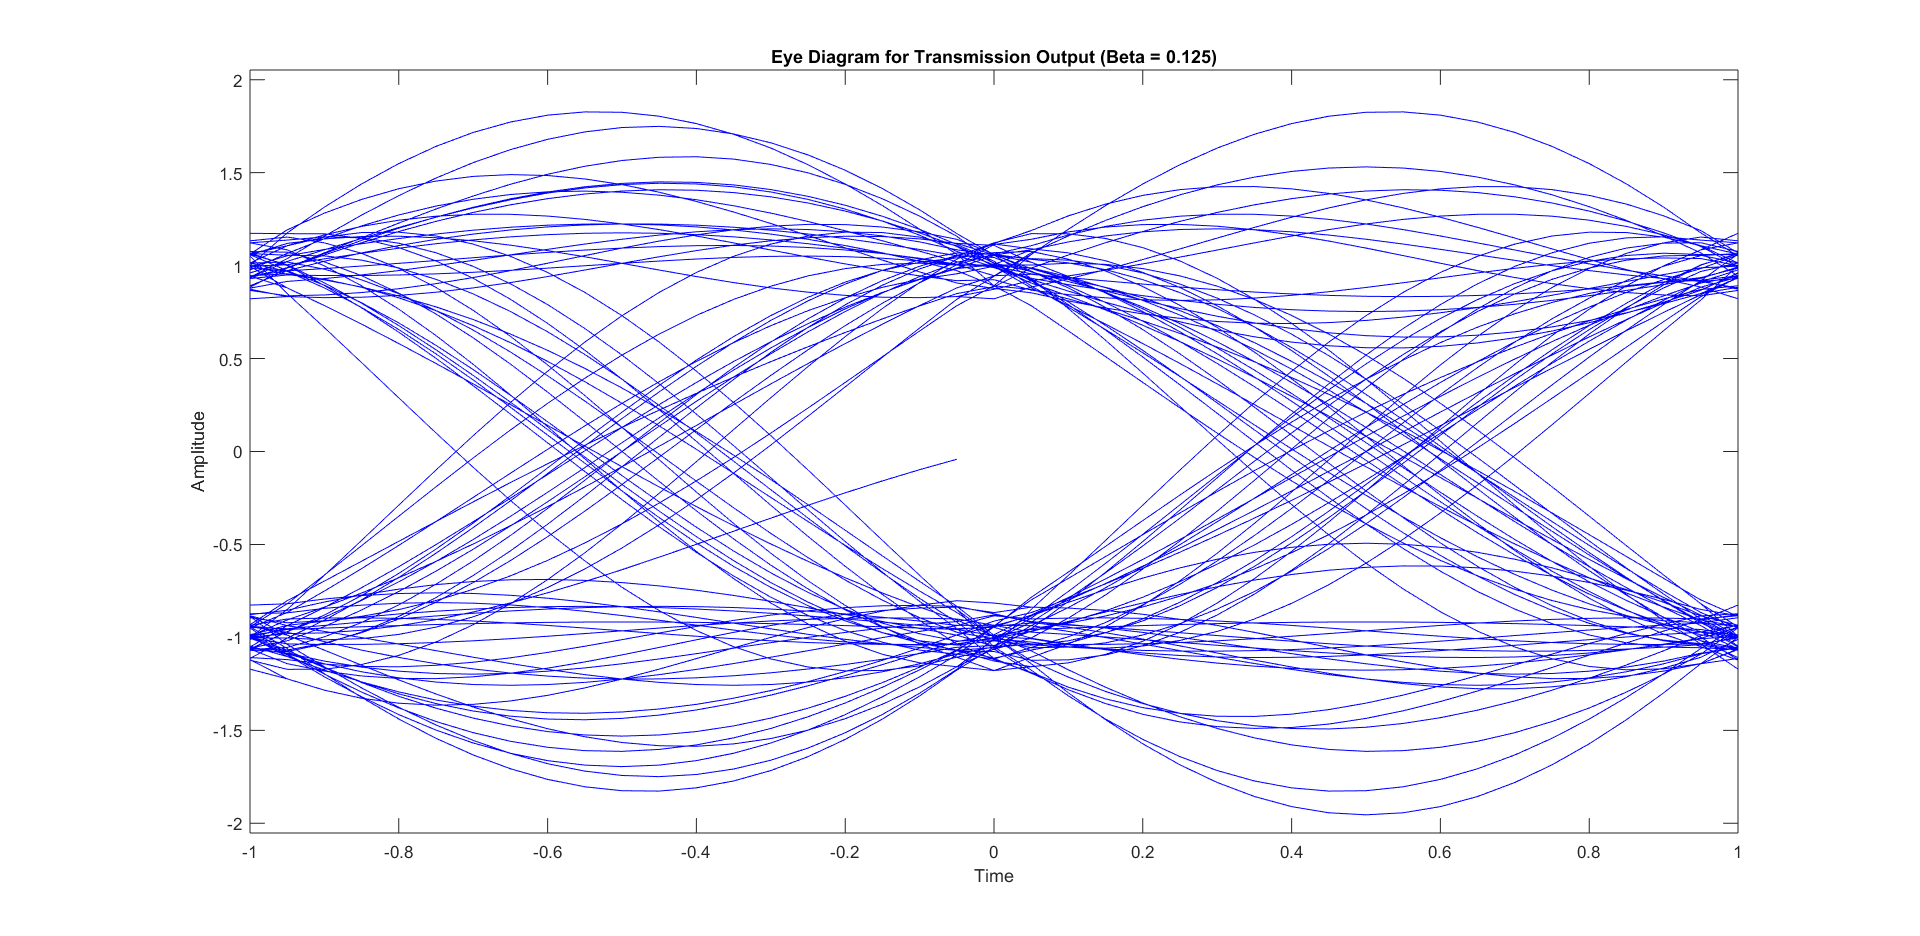
\includegraphics[width=0.65\textwidth]{img/eye_diagram_beta_125.png}
    \caption{Eye diagram $\beta = 0.125$}
  \end{center}
\end{figure}

\begin{figure}[h]
  \begin{center}

    \begin{subfigure}[b]{0.5\linewidth}
      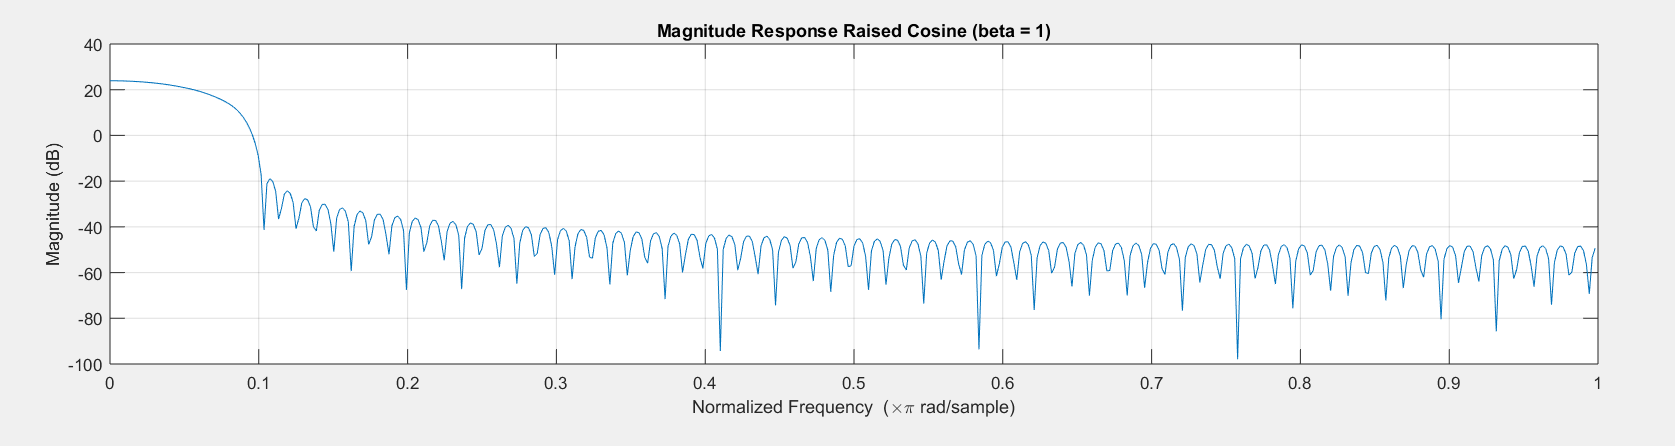
\includegraphics[width=\linewidth]{img/magnitude_response_beta_1.png}
      \caption{Magnitude Response $\beta = 1$}
    \end{subfigure}

    \begin{subfigure}[b]{0.5\linewidth}
      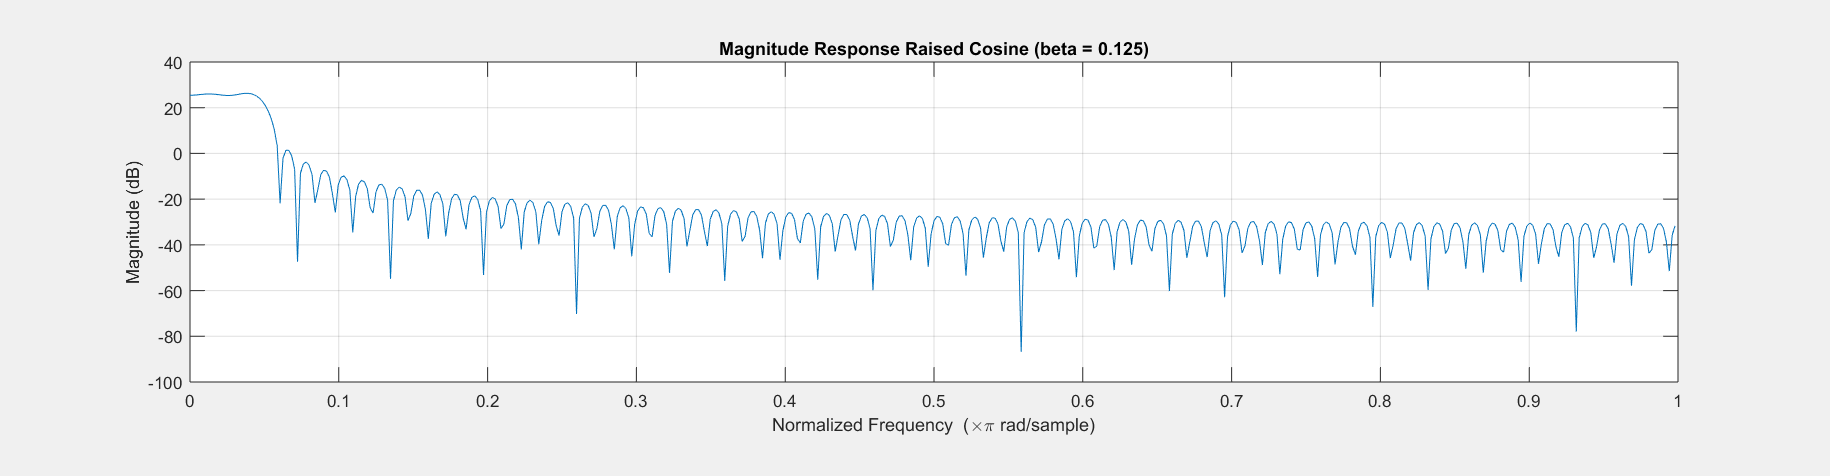
\includegraphics[width=\linewidth]{img/magnitude_response_beta_125.png}
      \caption{Magnitude Response $\beta = 0.125$}
    \end{subfigure}

  \end{center}
\end{figure}

\begin{figure}[h]
  \begin{center}

    \begin{subfigure}[b]{0.5\linewidth}
      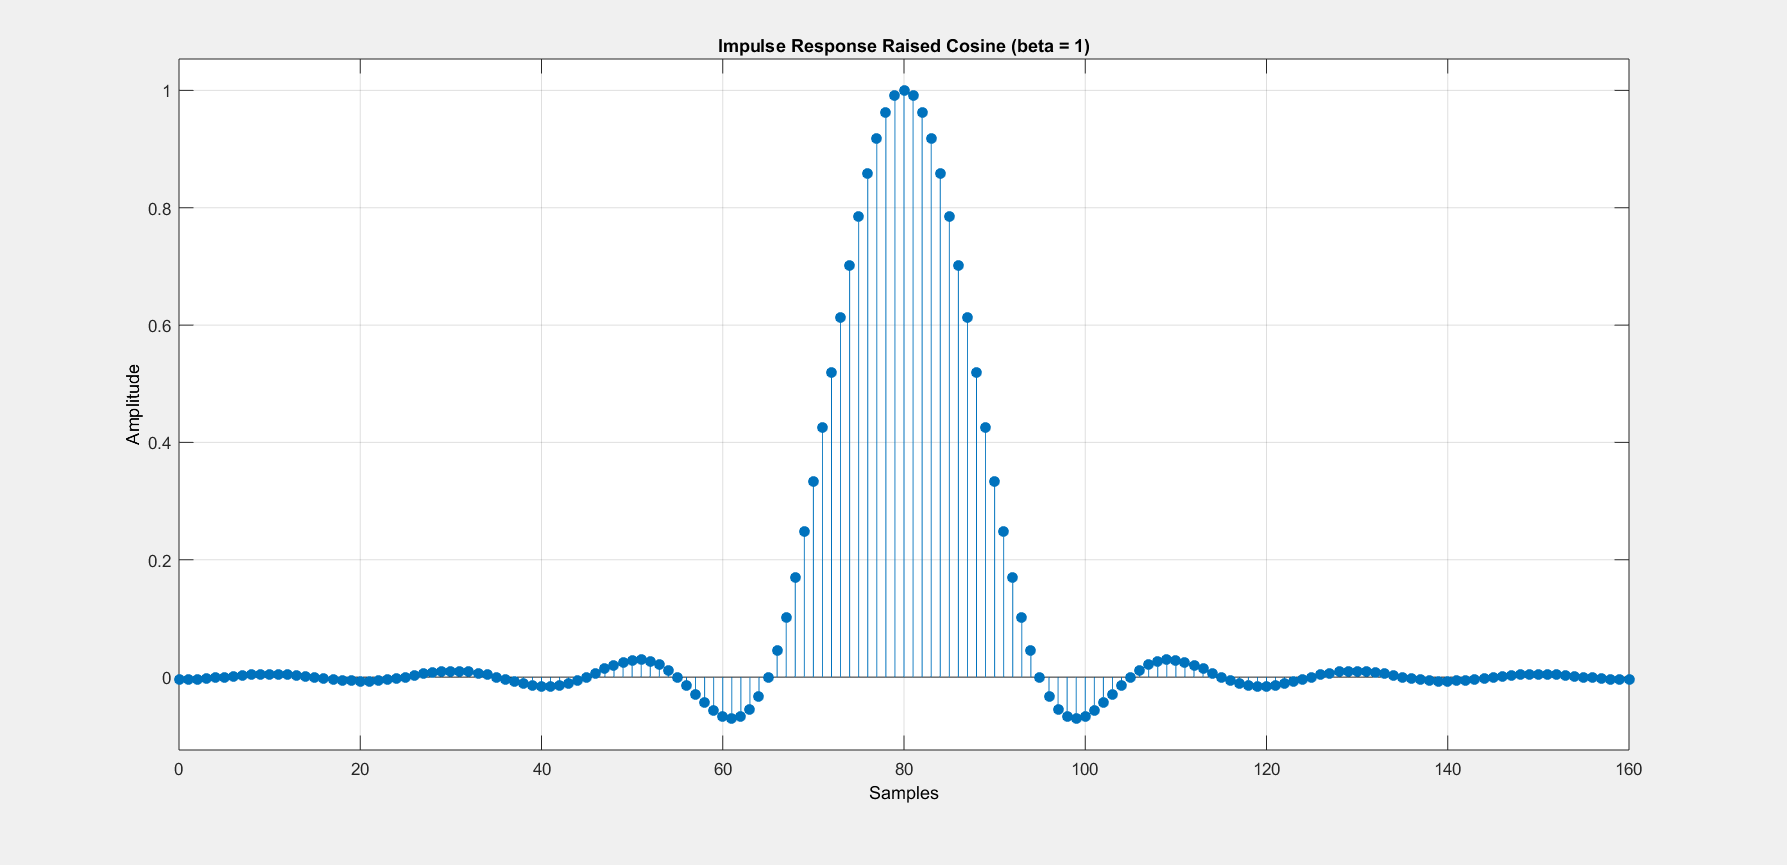
\includegraphics[width=\linewidth]{img/impulse_response_beta_1.png}
      \caption{Time Response $\beta = 1$}
    \end{subfigure}

    \begin{subfigure}[b]{0.5\linewidth}
      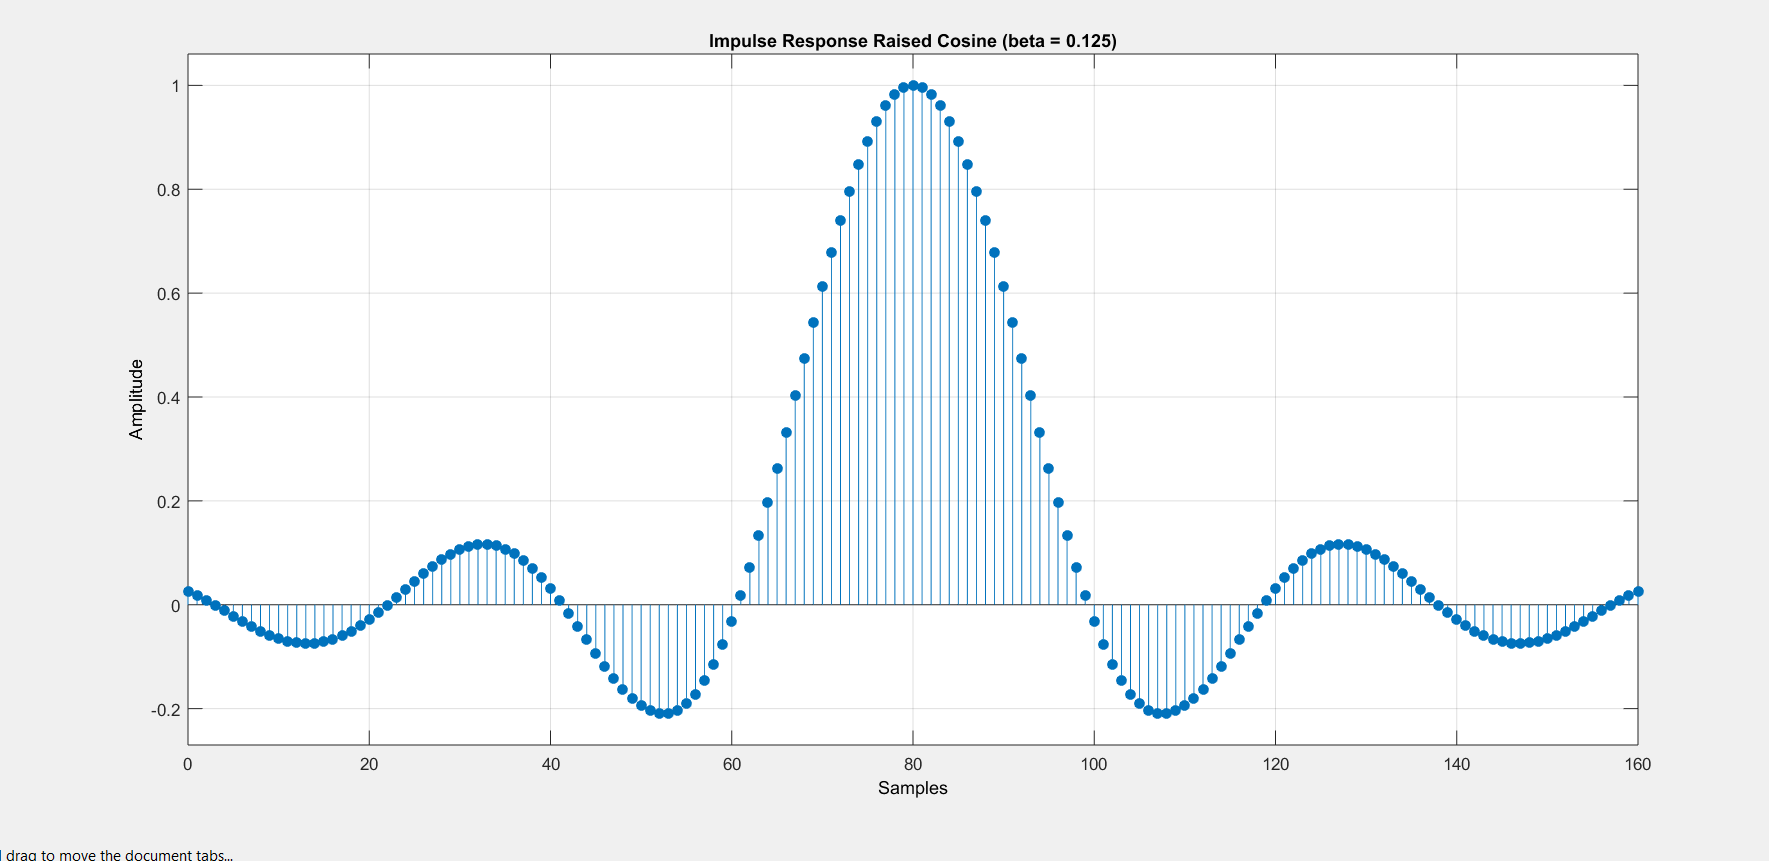
\includegraphics[width=\linewidth]{img/impulse_response_beta_125.png}
      \caption{Time Response $\beta = 0.125$}
    \end{subfigure}

  \end{center}
\end{figure}

Explain the major differences between the two filters with respect to their
	A) Magnitude responses 
	B) Impulse responses
2. What is the width of the impulse response for the =0.125 case? 
3. How would you obtain this number theoretically? (Hint: Look at the fsym and truncation limit you set)

\begin{figure}[h]
  \begin{center}

    \begin{subfigure}[b]{0.5\linewidth}
			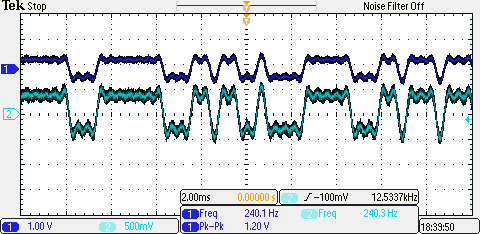
\includegraphics[width=0.65\textwidth]{img/DSK_implementation_beta_1.png}
      \caption{Time Response $\beta = 1$}
    \end{subfigure}

    \begin{subfigure}[b]{0.5\linewidth}
			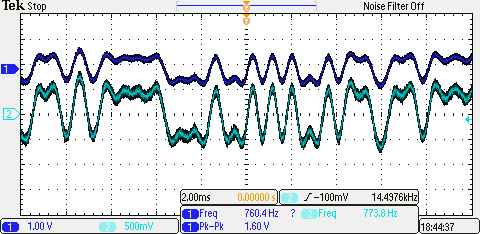
\includegraphics[width=0.65\textwidth]{img/DSK_implementation_beta_125.png}
      \caption{Time Response $\beta = 0.125$}
    \end{subfigure}

  \end{center}
\end{figure}

\subsection{Symbol Clock Recovery}

\textbf{Prefilter:}

\begin{center}
\begin{tabular}{c|c}
b0	&	 1				\\ \hline
b1	&  0				\\ \hline
b2	& -1				\\ \hline
-a1	&	 1.96004	\\ \hline
-a2	&	-0.984414 \\ \hline
\end{tabular}
\end{center}

\textbf{Bandpass:}

\begin{center}
\begin{tabular}{c|c}
b0	&	 1				\\ \hline
b1	&  0				\\ \hline
b2	& -1				\\ \hline
-a1	&	 1.87293\\ \hline
-a2	&	-0.969067\\ \hline
\end{tabular}
\end{center}

\begin{figure}[h]
  \begin{center}
    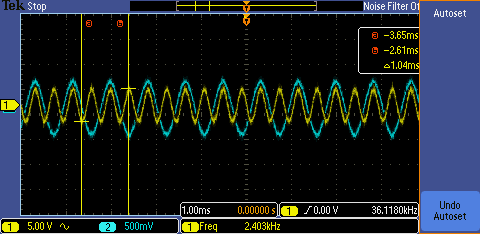
\includegraphics[width=0.65\textwidth]{img/dotting_sequence_SCR.png}
    \caption{Dotting sequence}
  \end{center}
\end{figure}

\begin{figure}[h]
  \begin{center}
    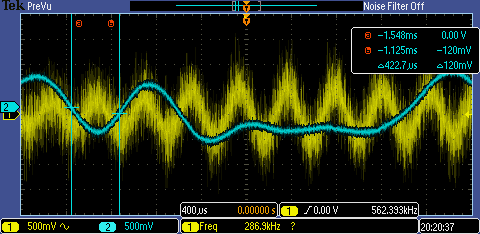
\includegraphics[width=0.65\textwidth]{img/2PAM_SCR.png}
    \caption{2-PAM SCR}
  \end{center}
\end{figure}

\pagebreak
\textbf{Code:}

\begin{verbatim}
	if (counter == 0) {
		symbol = SSRG_update(&SSRG_state); // pseudo random m-sequence
		x[0] = data[symbol]; // read the table

		/* dotting sequence
		symbol = symbol ^ 1;
		x[0] = data[symbol]; // read the table
		*/
	}

	// perform impulse modulation based on the FIR filter, B[N] 

	y  = 0;

	for (i = 0; i < 8; i++) {
		y +=  x[i]*B[counter + 20*i];	// perform the dot-product
	}

	if (counter == (samplesPerSymbol - 1)) {
		counter = -1; 

		/* shift x[] in preparation for the next symbol */

		for (i = 9; i > 0; i--) {
			x[i] = x[i - 1];          // setup x[] for the next input
		}
	}

	counter++;

	output = y;
	scr = clock_recover(y);
\end{verbatim}

\textbf{Table:}

\begin{center}
\begin{tabular}{c|c|c}
pattern	&	frequency & amplitude \\ \hline
dotted sequence	&	 2381 Hz	&	1.04 V				\\ \hline
dotted sequence	&	 2323 Hz	&	1.46 V				\\ \hline
\end{tabular}
\end{center}

\begin{figure}[h]
  \begin{center}
    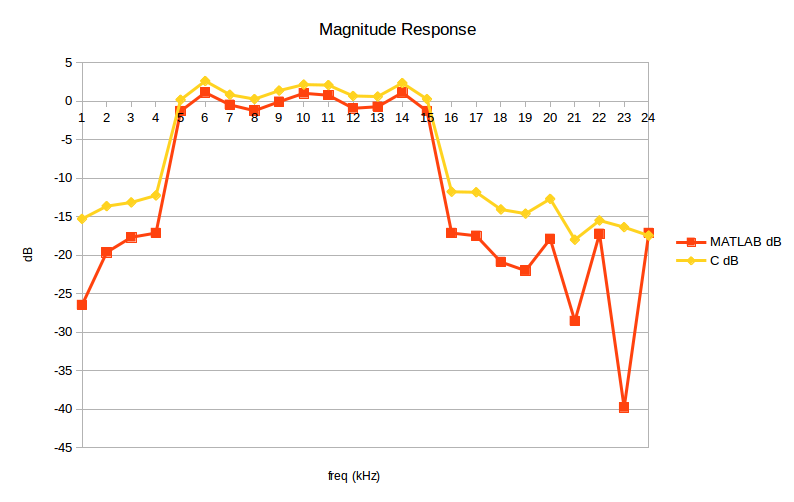
\includegraphics[width=0.65\textwidth]{img/fir_mag.png}
    \caption{FIR magnitude response.}
  \end{center}
\end{figure}

\textbf{Table:}
\begin{center}
\begin{tabular}{c|c|c|c}
freq (Hz)	& MATLAB dB	& C dB	& SOS dB \\ \hline
1  & 	-49.336911533	           &   -21.6164638623	   & -23.8559390512 \\ \hline
2  & 	-30.4835221116	         &   -18.9224923843	   & -22.8898454597 \\ \hline
3  & 	-18.5780755991	         &   -21.6164638623	   & -16.2092403443 \\ \hline
4  & 	-9.4231800523	           &   -16.4237176522	   & -8.3784900031  \\ \hline
5  & 	-3.0102999566	           &   -8.1242506928	   & -2.3578900898  \\ \hline
6  & 	-0.4907931843	           &   -2.1875730714	   & 0              \\ \hline
7  & 	-0.0431819157	           &   0	               & 0              \\ \hline
8  & 	-0.0013881395	           &   0.0008193849	     & 0              \\ \hline
9  & 	-0.000001107	           &   0.0016386925	     & 0              \\ \hline
10 &	-2.45915822097029E-06	   &   0.0024579228	     & 0              \\ \hline
11 &	-0.0012585765	           &   0.0032770759	     & 0              \\ \hline
12 &	-0.0255740552	           &   0.0040961518	     & 0              \\ \hline
13 &	-0.1988119832	           &   0.0049151504	     & 0              \\ \hline
14 &	-0.9408492775	           &   -0.5061173053	   & -0.5061173053  \\ \hline
15 &	-3.0102999566	           &   -2.4443175655	   & -2.7088828801  \\ \hline
16 &	-6.7158691567	           &   -4.9430922976	   & -6.1860504326  \\ \hline
17 &	-11.500586955	           &   -9.9793317575	   & -10.1886404311 \\ \hline
18 &	-16.8767672084	         &   -14.144850606	   & -15.595863949  \\ \hline
19 &	-22.8006774261	         &   -16.4237176522	   & -18.9224923843 \\ \hline
20 &	-29.5500422777	         &   -19.5217568519	   & -20.5061173053 \\ \hline
21 &	-37.7484943246	         &   -20.5061173053	   & -22.0205315841 \\ \hline
22 &	-48.8004344666	         &   -20.5061173053	   & -22.8898454597 \\ \hline
23 &	-67.1478923263	         &   -20.5061173053	   & -23.3594673767 \\ \hline
24 &	-77.232927344	           &   -20.5061173053	   & -23.8559390512 \\ \hline
\end{tabular}
\end{center}

\pagebreak

\textbf{Code:}

\begin{verbatim}
/*********Coefficients*************/
float B[N + 1] = {
    0.108499,	/* B[0] */
           0,	/* B[1] */
   -0.325498,	/* B[2] */
           0,	/* B[3] */
    0.325498,	/* B[4] */
           0,	/* B[5] */
   -0.108499,	/* B[6] */
};

float A[N + 1] = {
           1,	/* A[0] */
    -1.13553,	/* A[1] */
    0.944316,	/* A[2] */
   -0.637821,	/* A[3] */
    0.544417,	/* A[4] */
   -0.173657,	/* A[5] */
   0.0459008,	/* A[6] */
};
\end{verbatim}

\begin{verbatim}
/*********df_one*******************/
float sum = 0;
int i;

//dot product for numerator
for(i = 0; i < N + 1; i++)
{
		sum += B[i]*x[i];
}

//dot product for denominator
for(i = 1; i < N + 1; i++)
{
		sum -= A[i]*y[i];
}

y[0] = A[0]*sum;

//setup for next iteration
for(i = N; 0 < i; i--)
{
		x[i] = x[i - 1];
		y[i] = y[i - 1];
}
\end{verbatim}

\begin{verbatim}
/************SOS Coeff***************/
float SOS[SOS_SIZE][5] = {
{           1,            0,           -1,      1.28028,    -0.657254}, /* SOS[0] */
{           1,            0,           -1,    -0.513935,    -0.530466}, /* SOS[1] */
{           1,            0,           -1,     0.369184,    -0.131652}, /* SOS[2] */
};

float G[SOS_SIZE + 1] = {    0.4999,
                             0.4999,
                             0.4342,
                             1.0000};
\end{verbatim}

\begin{verbatim}
/************SOS*******************/
float biquad(int index, float value)
{
	x[index][0] = value;
	float ret_val = SOS[index][0]*x[index][0] + SOS[index][1]*x[index][1] + 
  SOS[index][2]*x[index][2] +
	SOS[index][3]*y[index][1] + SOS[index][4]*y[index][2];

	y[index][0] = ret_val;

	x[index][2] = x[index][1];
	x[index][1] = x[index][0];

	y[index][2] = y[index][1];
	y[index][1] = y[index][0];

	return ret_val;
}
\end{verbatim}

%----------------------------------------------------------------------------------------
%	SECTION 4
%----------------------------------------------------------------------------------------

\section{Discussion}

\subsection{Linear and Circular buffering}

We learned that the MATLAB fda tool is very good for quickly designing filters.
After examining the magnitude plot in MATLAB we got a good idea about what to expect from the real time implementation.

\subsection{Frame based processing}

One big take away was that the compiler is a way better optimizer than we are.
Also we realized that some compiler optimizations lead to very hard to understand assembly code.

\subsection{IIR filtering}

It was a surprise that the IIR filter achieved such great performance with far less filter coefficients.
Also it was interesting to see the effect of using incorrect gains in the cascuade of biquads.

%----------------------------------------------------------------------------------------
%	SECTION 5
%----------------------------------------------------------------------------------------

\section{Answers to questions}

\begin{enumerate}
  \begin{item}
    Number of taps before you run out of time for FIR filtering.

  \textbf{Answer:}
    For an arbitrary processor using a circular buffer to implement an FIR filter, where $m$ is the time it takes for a multiply to complete and $a$ is the time it takes for an addition to complete.
    We would want our processing to take less than our sampling period $T_s$.
    So for an FIR filter with $N$ coefficients we  would have $N$ multiply and $N - 1$ add opperations.

    \begin{equation}
      T_s > mN + a(N - 1)
    \end{equation}

    Solving for $N$ we arrive at this constraint for the maximum number of taps.

    \begin{equation}
      \frac{T_s + a}{m + a} > N
    \end{equation}
  \end{item}

  \begin{item}
    Why use circular buffers?

  \textbf{Answer:}
    Using a circular buffer eliminates the time needed to shift values using a linear buffer implementation, which would scale shifts linearly.

  \end{item}

  \begin{item}
    What happens if you do not multiply the scale factor in an IIR filter implementation using a cascade of second-order sections (SOS)?

  \textbf{Answer:}
    If we do not multiply by a scaling factor our system may be unstable.
    When we design a transfer function we use a set of specifications to guide our choices of poles and zeros.
    From this set of poles and zeros we arrive at a single section implementation.
    To create a more practical implementation we instead break our single section into many second order sections.
    As a result of factoring our large polynomial into many second order polynomials we get a set of scaling factors between each section.
    By ignoring these scaling factors, we would essentially change the location of the poles and zeros, and by extent the response of the entire filter.
  \end{item}

  \begin{item}
    Advantages and disadvantages of FIR vs. IIR filters. 

  \textbf{Answer:}

    \textbf{FIR}

    \textit{Pros:}

    \begin{itemize}
      \item Linear phase
      \item BIBO stability
    \end{itemize}

    \textit{Cons:}

    \begin{itemize}
      \item Large number of coefficients
    \end{itemize}

    \textbf{IIR}

    \textit{Pros:}

    \begin{itemize}
      \item Low number of Coefficients
    \end{itemize}

    \textit{Cons:}

    \begin{itemize}
      \item May become unstable
      \item non linear phase
    \end{itemize}

  \end{item}

\end{enumerate}

%----------------------------------------------------------------------------------------
%	BIBLIOGRAPHY
%----------------------------------------------------------------------------------------

\bibliography{mybib}
\bibliographystyle{plain}

%----------------------------------------------------------------------------------------


\end{document}
